% Copy this file to start a new note. Builds with pdflatex (the default recipe).
\documentclass[11pt]{article}
\usepackage{quicknotes}

\title{Data Science 6}
\author{Mark}
\date{}

\begin{document}
\maketitle

% \lecture{number}{date}{topic}
\lecture{5}{Monday, June 30, 2026}{Day 5}
You can populate a table with $\text{with\_columns}$ using the name and array. Note a objects function vs an attribute.

You can extract rows from a table by
\begin{enumerate}
    \item tbl.where() by condtion
    \item tbl.take() by index
\end{enumerate}

for \textbf{tbl.take()} use \textbf{np.arange()} ex: \textbf{table.take(np.arrange(5))}. np.arrange works by returing an array usal start step but stop is not included in the array.
\begin{note}
    \itshape Must have all postional arguments or all keyword arguments
\end{note}

\section{Booleans}

boolean predicates use the "are." Usally can just use lambda functions
Recall the comparsion operators from earlier 

\begin{figure}[h]
    \centering
    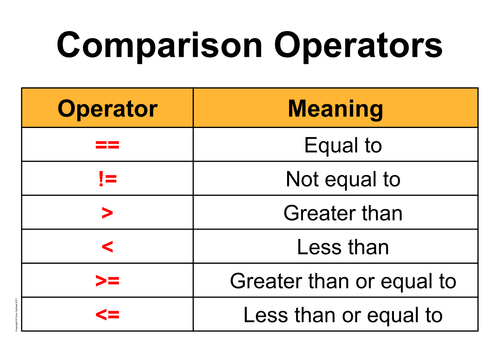
\includegraphics[width=0.7\textwidth]{image6.png}
    \caption{Python Ops}
    \label{fig:label}
\end{figure}

Falsey Values:

    \begin{enumerate}
        \item False
        \item 0
        \item 0.0
        \item "" (empty string)
        \item None
    \end{enumerate}

Everything else is Truthy. int(True) = 1

\begin{note}
    \itshape Dont compare floates using == because of floating point error. and use instead \textbf{abs(0.1 * 6 - 0.6) $<$ 0.0001}
\end{note}

\section{Functions}
Recall how to make a function. can use a doc string if feeling like you have time to waste

Recall string methods

\begin{figure}[h]
    \centering
    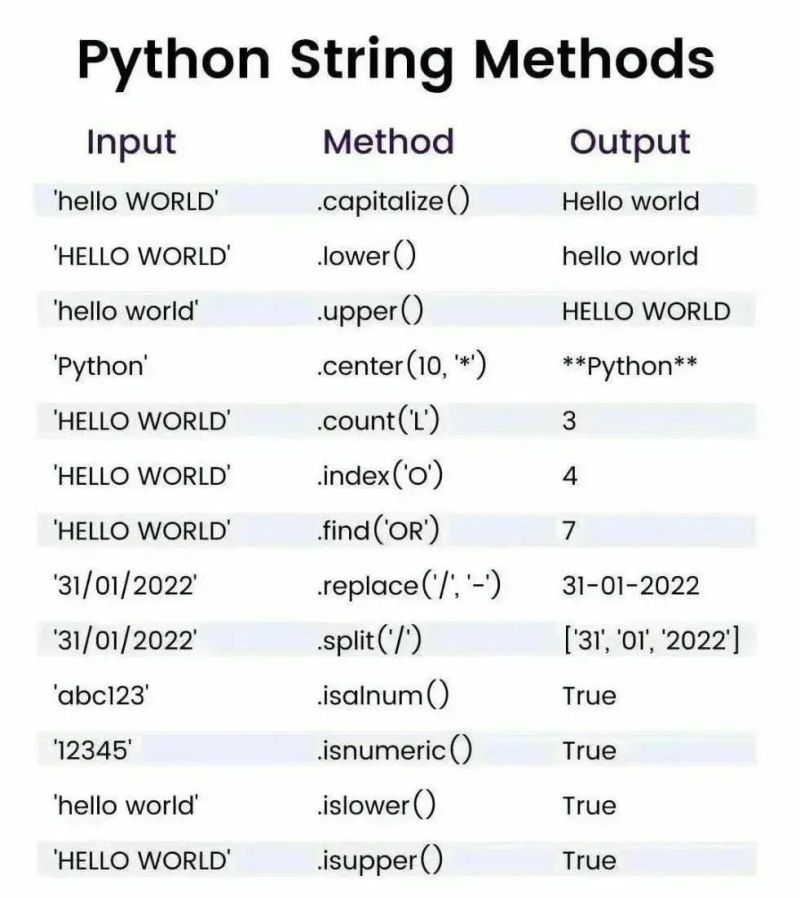
\includegraphics[width=0.7\textwidth]{image7.png}
    \caption{String Methods}
    \label{fig:label}
\end{figure}
\end{document}
